\section{Testy rozwiązania}
	\label{final:testy}

	\subsection{Generowanie grafów}
		\label{final:testy:generowanie}

		Istotnym etapem projektu było przygotowywanie danych testowych. Do tego celu został zaimplementowany generator grafów (klasa \texttt{GraphGenerator}). Generowane grafy były zapisywane do pliku w celu ich późniejszego wykorzystania do analizy. Najwięcej czasu, bo przez około cztery dni, generowaliśmy grafy, natomiast ich analiza (obliczanie maksymalnych składowych spójnych etc.), zajęła nam niecały dzień. Grafy, które zostały wygenerowane, w postaci skompresowanej zajęły około 10 GB pamięci na dysku.

		Utworzone zostało znacznie więcej grafów, niż których poddano analizie. Wynikło to głównie z faktu, iż grafy euklidesowe stają się bardzo szybko spójne (to znaczy, że niewielka zmiana promienia powoduje gwałtowne zmiany odnośnie spójności), co zostało odkryte dopiero po ich wygenerowaniu.

		Podsumowując, zostały wygenerowane następujące zestawy grafów:
		\begin{itemize}
			\item Rozmiary od 100 do 2000 z krokiem 100 oraz promienie od 0,001 do 1,0 z krokiem 0,001
			\item Rozmiar 10000 oraz promienie od 0,01 do 0,05 z krokiem 0,001
		\end{itemize}

		W ramach każdego zestawu tworzone było łącznie sto grafów. Okazała się to być ilość optymalna, zarówno pod kątem czasu obliczeń, jak i cech losowych otrzymywanych grafów.

	\subsection{Przeprowadzone testy}
		\label{final:testy:przyklad1}

		Dla wygenerowanych grafów badaliśmy głównie trzy parametry:
		\begin{itemize}
			\item Rozmiary największych składowych spójnych
			\item Średni rozmiar największej składowej spójnej - suma rozmiarów największych składowych spójnych podzielona przez ilość grafów (czyli 100 dla każdego z przypadków)
			\item Prawdopodobieństwo spójności - ilość grafów spójnych (czyli takich, dla których rozmiar największej składowej spójnej równa się rozmiarowi grafu) podzielona przez łączną ilość grafów dla danego przypadku (czyli 100)
		\end{itemize}

		Na rysunkach~\ref{500-0_0010_125_consistency_prob},~\ref{500-0_0010_125_max_comps_sizes_means},~\ref{2000-0_06_0-consistency_prob},~\ref{2000-0_06_0-max_comps_sizes_means},~\ref{10000-0_0:3_0-consistency_prob} oraz ~\ref{10000-0_0:3_0-max_comps_sizes_means} przedstawiliśmy analizę prawdopodobieństwa spójności oraz rozmiaru największej składowej spójnej dla grafów o rozmiarach od 300 do 1000, 2000 oraz 10000. Na rysunkach~\ref{500-max_comps_sizes},~\ref{2000-max_comps_sizes},~\ref{10000-max_comps_sizes} zaś przedstawiliśmy rozkład rozmiarów największych składowych spójnych dla trzech wybranych rozmiarów grafów: 500, 2000 oraz 10000.

		\begin{figure}[h!]
			\centering
			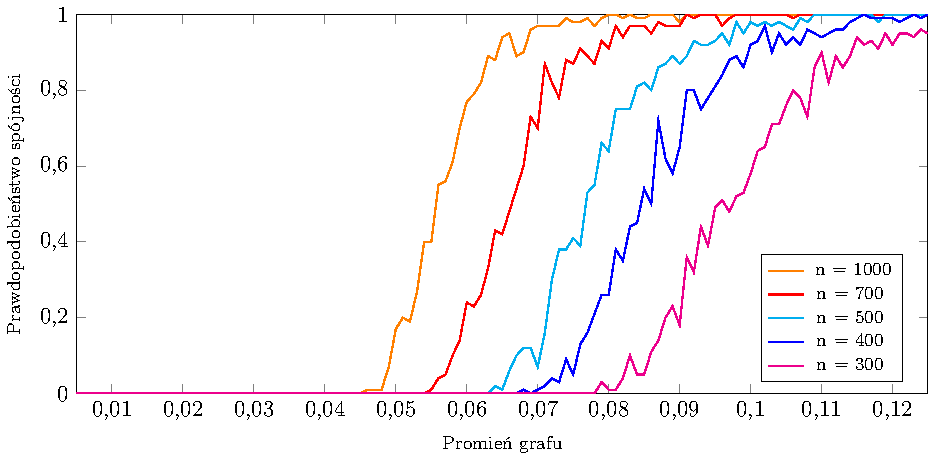
\includegraphics[scale=0.8]{500-0_0010_125_consistency_prob.pdf}
			\caption{Prawdopodobieństwo spójności grafów o rozmiarach od 300 do 1000 i zmieniającym się promieniu}
			\label{500-0_0010_125_consistency_prob}
		\end{figure}

		\begin{figure}
			\centering
			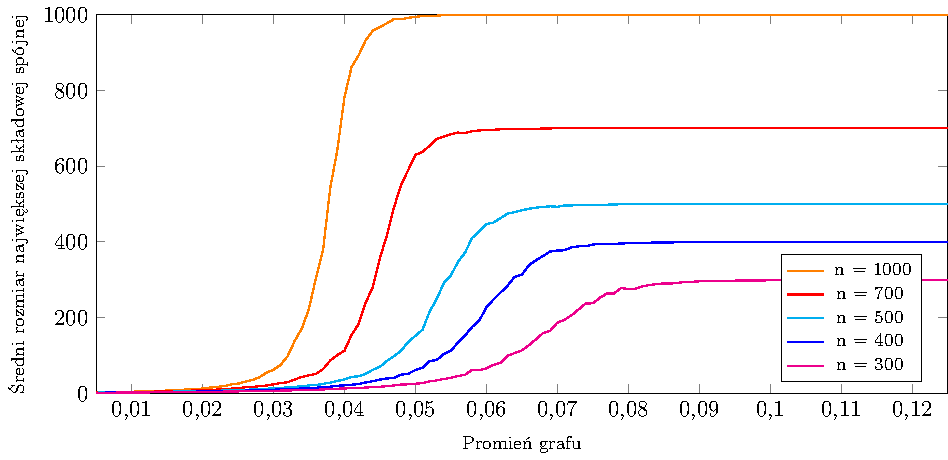
\includegraphics[scale=0.8]{500-0_0010_125_max_comps_sizes_means.pdf}
			\caption{Średni rozmiar największej składowej spójnej dla grafów o rozmiarach od 300 do 1000 i zmieniającym się promieniu}
			\label{500-0_0010_125_max_comps_sizes_means}
		\end{figure}

		\begin{figure}
			\centering
			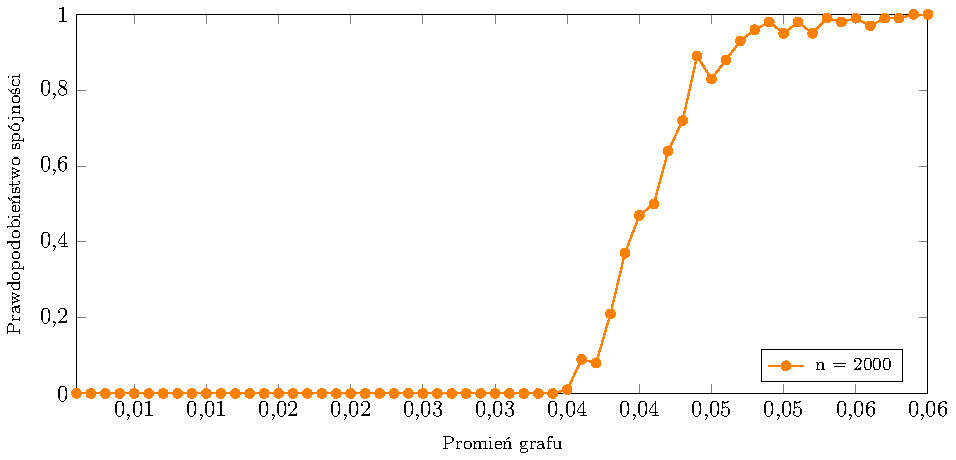
\includegraphics[scale=0.8]{2000-0_06_0-consistency_prob.pdf}
			\caption{Prawdopodobieństwo spójności grafu o rozmiarze 2000 i zmieniającym się promieniu}
			\label{2000-0_06_0-consistency_prob}
		\end{figure}

		\begin{figure}
			\centering
			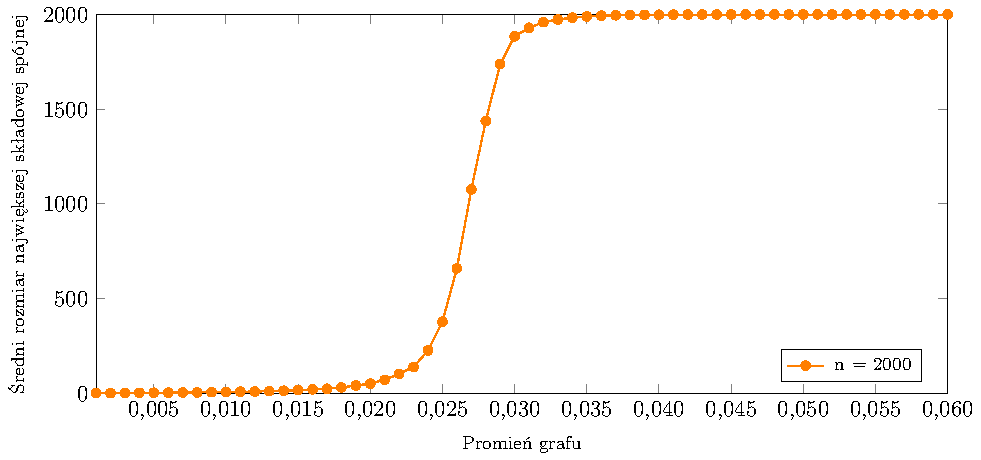
\includegraphics[scale=0.8]{2000-0_06_0-max_comps_sizes_means.pdf}
			\caption{Średni rozmiar największej składowej spójnej dla grafu o rozmiarze 2000 i zmieniającym się promieniu}
			\label{2000-0_06_0-max_comps_sizes_means}
		\end{figure}

		\begin{figure}
			\centering
			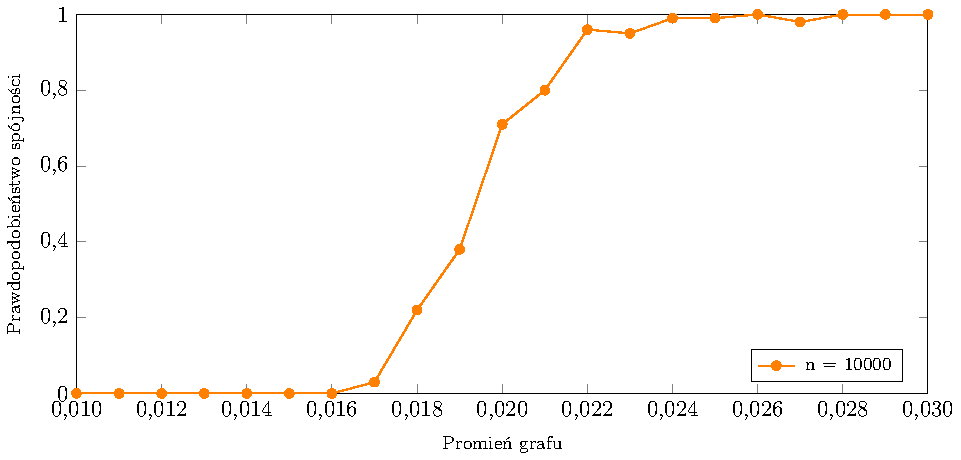
\includegraphics[scale=0.8]{10000-0_0:3_0-consistency_prob.pdf}
			\caption{Prawdopodobieństwo spójności grafu o rozmiarze 10000 i zmieniającym się promieniu}
			\label{10000-0_0:3_0-consistency_prob}
		\end{figure}

		\begin{figure}
			\centering
			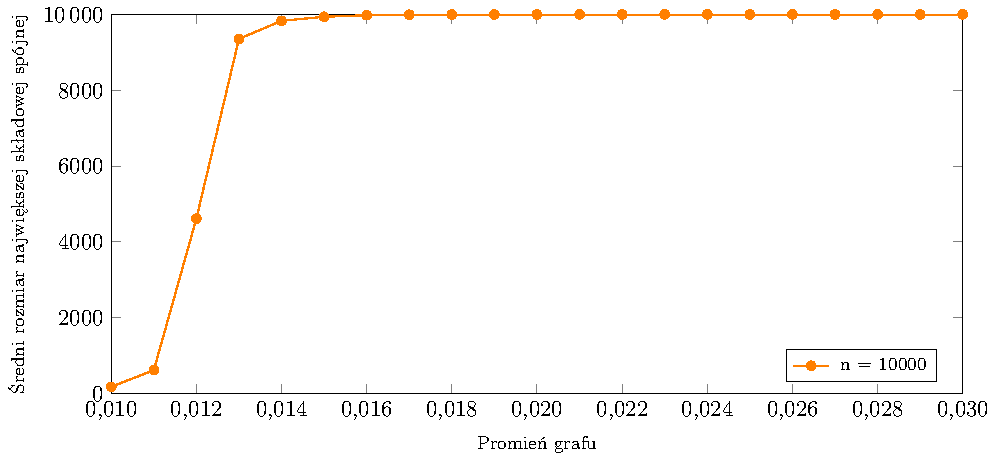
\includegraphics[scale=0.8]{10000-0_0:3_0-max_comps_sizes_means.pdf}
			\caption{Średni rozmiar największej składowej spójnej dla grafu o rozmiarze 10000 i zmieniającym się promieniu}
			\label{10000-0_0:3_0-max_comps_sizes_means}
		\end{figure}

		\begin{figure}
			\centering
			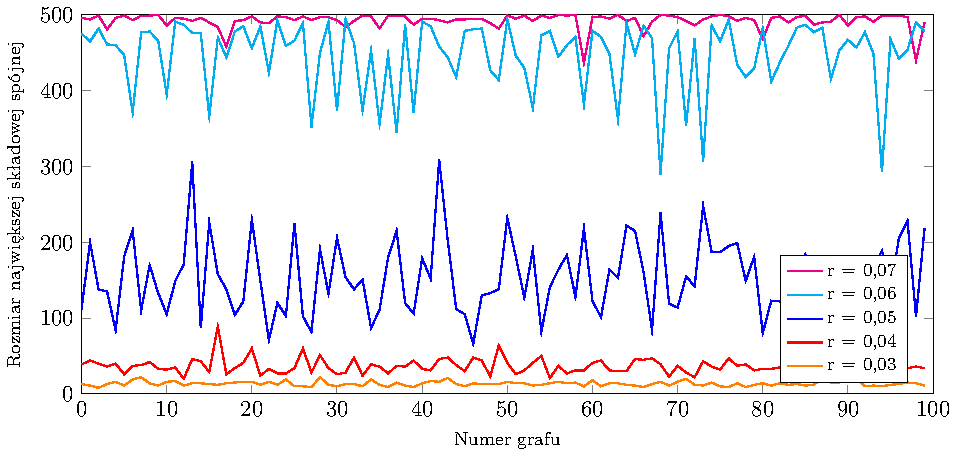
\includegraphics[scale=0.8]{500-max_comps_sizes.pdf}
			\caption{Rozmiary największych składowych spójnych dla 100 grafów o rozmiarze 500 i zmieniającym się promieniu}
			\label{500-max_comps_sizes}
		\end{figure}

		\begin{figure}
			\centering
			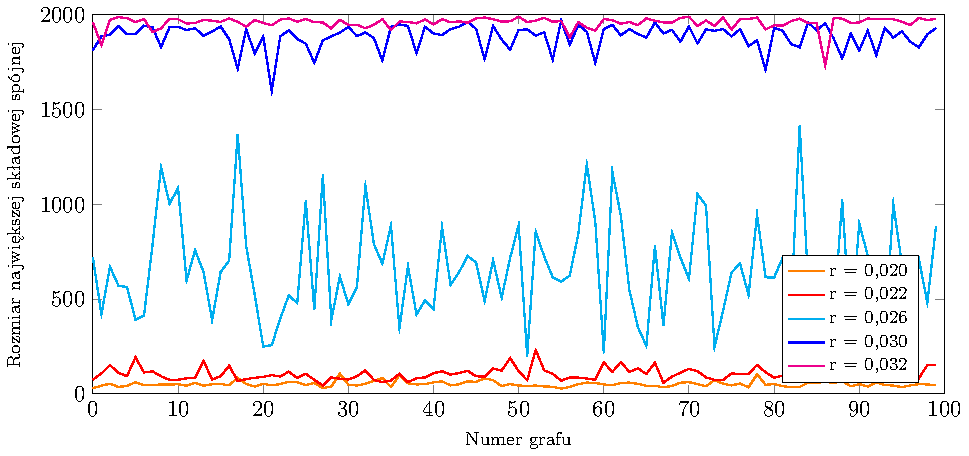
\includegraphics[scale=0.8]{2000-max_comps_sizes.pdf}
			\caption{Rozmiary największych składowych spójnych dla 100 grafów o rozmiarze 2000 i zmieniającym się promieniu}
			\label{2000-max_comps_sizes}
		\end{figure}

		\begin{figure}
			\centering
			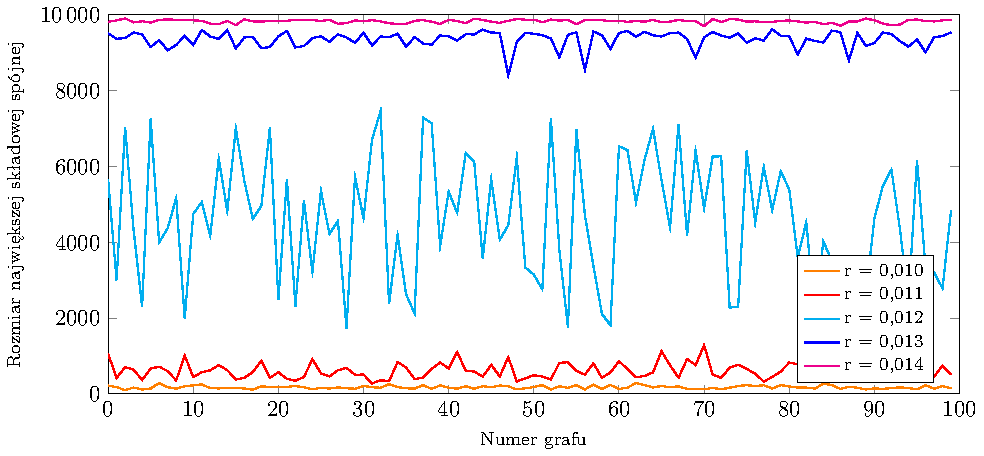
\includegraphics[scale=0.8]{10000-max_comps_sizes.pdf}
			\caption{Rozmiary największych składowych spójnych dla 100 grafów o rozmiarze 10000 i zmieniającym się promieniu}
			\label{10000-max_comps_sizes}
		\end{figure}
>>>>>>> Final version

	\subsection{Wnioski}
		\label{final:testy:wnioski}

		Z zamieszczonych rysunków można zauważyć, że wraz że wraz ze wzrostem liczby wierzchołków grafu rośnie również prawdopodobieństo, że będzie on spójny. Podobna zależność występuje przy zmianie promienia. Warto również wspomnieć o tym, że przy małej liczbie wierzchołków oraz małemu promieniowi prawdopodobieństwo spójności jest zerowe. W pewnym momencie następuje nagły wzrost prawdopodobieństa i rośnie ono dosyć szybko. Następnie zwalnia na poziomie 90 procent i powoli dąży do maksymalnej wartości.

		W skrócie z przeprowadzonych testów można wyciągnąć następujące wnioski:
		\begin{itemize}
			\item Wraz ze wzrostem liczby wierzchołków rośnie prawdopodobieństwo spójności sieci
			\item Wraz ze wzrostem promienia rośnie prawdopodobieństwo spójności sieci
			\item Im większa liczba wierzchołków w grafie tym większy średni rozmiar największej składowej spójnej
			\item Im większy promień grafu tym większy średni rozmiar największej składowej spójnej
		\end{itemize}
